\documentclass{article}
\usepackage[bottom]{footmisc}
\usepackage{graphicx}
\usepackage{float}
%\usepackage{adjustbox}
\newcommand{\V}{\verb}
\newcommand{\x}{$\textbf{X}$}
\newcommand{\y}{$\textbf{Y}$}
\newcommand{\s}{$\textbf{S}$}
\newcommand{\A}{$\textbf{A}$}
\newcommand{\mx}{$\textbf{M}_{\textbf{X}}$}
\newcommand{\my}{$\textbf{M}_{\textbf{Y}}$}
\newcommand{\ma}{$\textbf{M}_{\textbf{A}}$}
\newcommand{\q}{$\textbf{Q}_{\textbf{1}}$}
\newcommand{\qq}{$\textbf{Q}_{\textbf{2}}$}
\newcommand{\pc}{$\textbf{PC}$}    
\newcommand{\J}{$\textbf{J}$}
\renewcommand{\thefootnote}{\roman{footnote}}


\title{FML: a VM implemented in SML}
\author{Henrik Sommerland, Oskar Ahlberg, Aleksander Lunqvist}
\date{\today}

\begin{document}
\maketitle
\section{Introduction}
For our project we have decided to build a virtual 
machine(VM) in SML.
The name FML is just an arbitrary thre letter name and has no meaning or interpertation.
The VM is a RISC machine using a Von-Neuman architecture. It has a very
minimalistic instruction set. The design of FML resembles those of older 8-bit
architectures such as the MOS 6510 and the Z80 microprocessors commonly in use
during the late 70s and early 80s. The FML machine has no ``bus width'' and 
works exclusivley with signed integers\footnote{The details of the integers
used are dependent on which SML implementation is used}. The lack of a physical
bus enables the VM to do things wich an ordinary CPU could not achive such as
reading from two registers at the same time. Even though
the cpu have very few operations (only 27) a very effective instruction set architecture
makes these operations very flexibels and there are roughly 600 valid    
instruction codes. It is also noteworthy that FML is asycrounous and has now
predefined clock frequenzy.\footnote{Allthogh for debugging purposues one can
use both manual stepping and a fixed update speed.}

So even though FML is a very minimalistic machine it is quite powerfull.
We have allso built a fully featured assembler for the FML machine.
\section{The VM}
Here a informal description of the workings of the machine. For a more detailed
description se the VM specifications in the appendix.
\subsection{General}
The FML machine is built up as a very simple von-neuman architecture. The
machine consists ony of a few major components. It's notewhorthy that there is
no instruction decoder present. This is since all of the instruction decoding
and handling takes place within the software implementation of the machine.
The size of the memory the machine has avaliable is arbitrary and is defined at
the initilazion of the machine. Below will follow a dataflow diagram of the
machine, describing all of the components and how they can communicate.  

\begin{figure}[H]
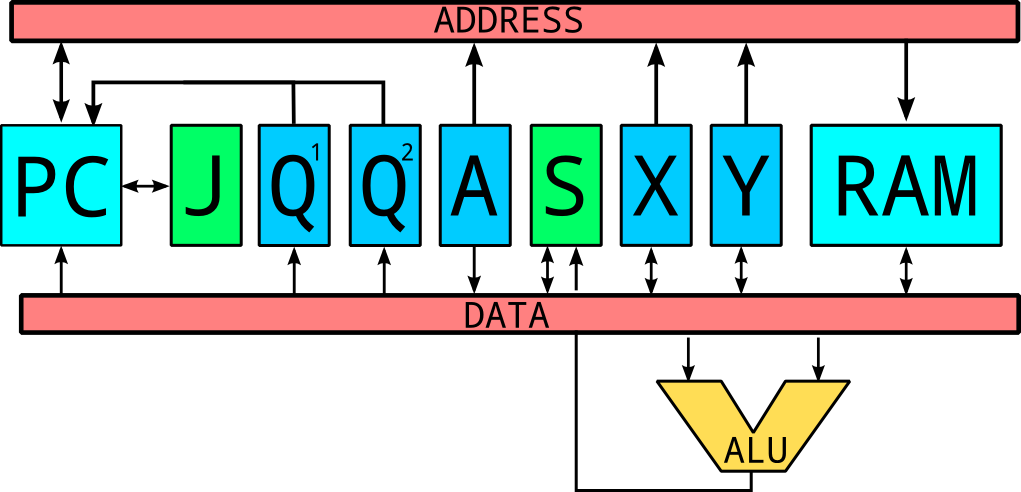
\includegraphics[width=\textwidth,height=\textheight,keepaspectratio]{Dataflow.png}
\caption{Dataflow diagram of the FML machine}
\end{figure}       

Now this image might be a little bit confusing. One should consider the two read
rectangles DATA and ADDRESS as ``viritual buses''. One can interpret the picture
as: X can both read and write from other components and be used for addressing.
Below will follow brief descriptions of the components. More indepth
descriptions are given in the appendix.

\begin{description}
  \item[X and Y] \hfill \\ 
  These are the two general purpose registers wich can be read,
  written to and used for addressing.
  \item[S] \hfill \\
  This is the general purpose stack. It can be both read and
  written to. Everytime some thing gets written to the stack it gets pushed onto the
  stack and everytime something is read from the stack the stack gets popped.
  The stack can not be used for addressing.
  \item[A] \hfill \\
  This is only a virtual register. It is read only and can be used for
  addressing. This is only used if an instructuion uses a non-register
  argument\footnote{A non-registry argument is a argument wich is not any of
  the registers, the stack, or something from the memmory. The value of A will
  (if used) be at the memmory cell directly folowing the one at wich the
  program counter is.}.
  \item[Q$^1$ and Q$^2$] \hfill \\
  These are the two interupt registers. These are very special and can only be
  written to. They will hold the adresses to wich the machine should jump if an
  prepherial component makes a interupt request. More on this later.
  \item[PC]\hfill \\
  This is the program counter. It keeps track on where in the memmory the 
  instructions are being read from. It allso handles the jumping.
  \item[J]\hfill \\
  This is the jump stack. This stack is used to store the return addresses for
  subroutine jumps. This stack can only be manipulated by the program counter.
  \item[ALU]\hfill \\
  This is not really a ALU. The machine does not have a seppareta ALU component
  but this is just here to illustrate that the all of the components which can
  be read from can be used as arguments for arithmetic and logical operations.
  All of the results from the arithmetic and logical operations are always put
  on the stack.
  \item[RAM]\hfill \\
  This is the random access memmory of the machine.
\end{description}

\subsection{Instruction Set Architecture}
The


\end{document}
